
%(BEGIN_QUESTION)
% Copyright 2014, Tony R. Kuphaldt, released under the Creative Commons Attribution License (v 1.0)
% This means you may do almost anything with this work of mine, so long as you give me proper credit

Test leads for DC voltmeters are usually just two individual lengths of wire connecting the meter to a pair of probes.  For highly sensitive instruments, a special type of two-conductor cable called {\it coaxial cable} is generally used instead of two individual wires.  Coaxial cable -- where a center conductor is ``shielded'' by an outer braid or foil that serves as the other conductor -- has excellent immunity to induced ``noise'' from electric and magnetic fields:

$$\includegraphics[width=15.5cm]{i00844x01.eps}$$

\filbreak

When measuring high-frequency AC voltages, however, the parasitic capacitance and inductance of the coaxial cable may present problems.  We may represent these distributed characteristics of the cable as ``lumped'' parameters: a single capacitor and a single inductor modeling the cable's behavior:

$$\includegraphics[width=15.5cm]{i00844x02.eps}$$

Typical parasitic values for a 10-foot cable would be 260 pF of capacitance and 650 $\mu$H of inductance.  The voltmeter itself, of course, is not without its own inherent impedances, either.  For the sake of this example, let's consider the meter's ``input impedance'' to be a simple resistance of 1 M$\Omega$.

Calculate what voltage the meter would register when measuring the output of a 20 volt AC source, at these frequencies:

\begin{itemize}
\item{} $f =$ 1 Hz ; $V_{meter} =$
\item{} $f =$ 1 kHz ; $V_{meter} =$
\item{} $f =$ 10 kHz ; $V_{meter} =$
\item{} $f =$ 100 kHz ; $V_{meter} =$
\item{} $f =$ 1 MHz ; $V_{meter} =$
\end{itemize}

\underbar{file i00844}
%(END_QUESTION)





%(BEGIN_ANSWER)

There is no need to express your answers in complex-number form, since an analog voltmeter does not register the phase angle of the measured voltage:

\begin{itemize}
\item{} $f =$ 1 Hz ; $V_{meter} =$ 20 V
\item{} $f =$ 1 kHz ; $V_{meter} =$ 20 V
\item{} $f =$ 10 kHz ; $V_{meter} =$ 20.01 V
\item{} $f =$ 100 kHz ; $V_{meter} =$ 21.43 V
\item{} $f =$ 1 MHz ; $V_{meter} =$ 3.526 V
\end{itemize}

%(END_ANSWER)





%(BEGIN_NOTES)


%INDEX% Electronics review: AC reactance and impedance
%INDEX% Electronics review: series-parallel AC circuits

%(END_NOTES)

